% !TEX root = ./docs.tex




\begin{figure}[h]
    \centering
    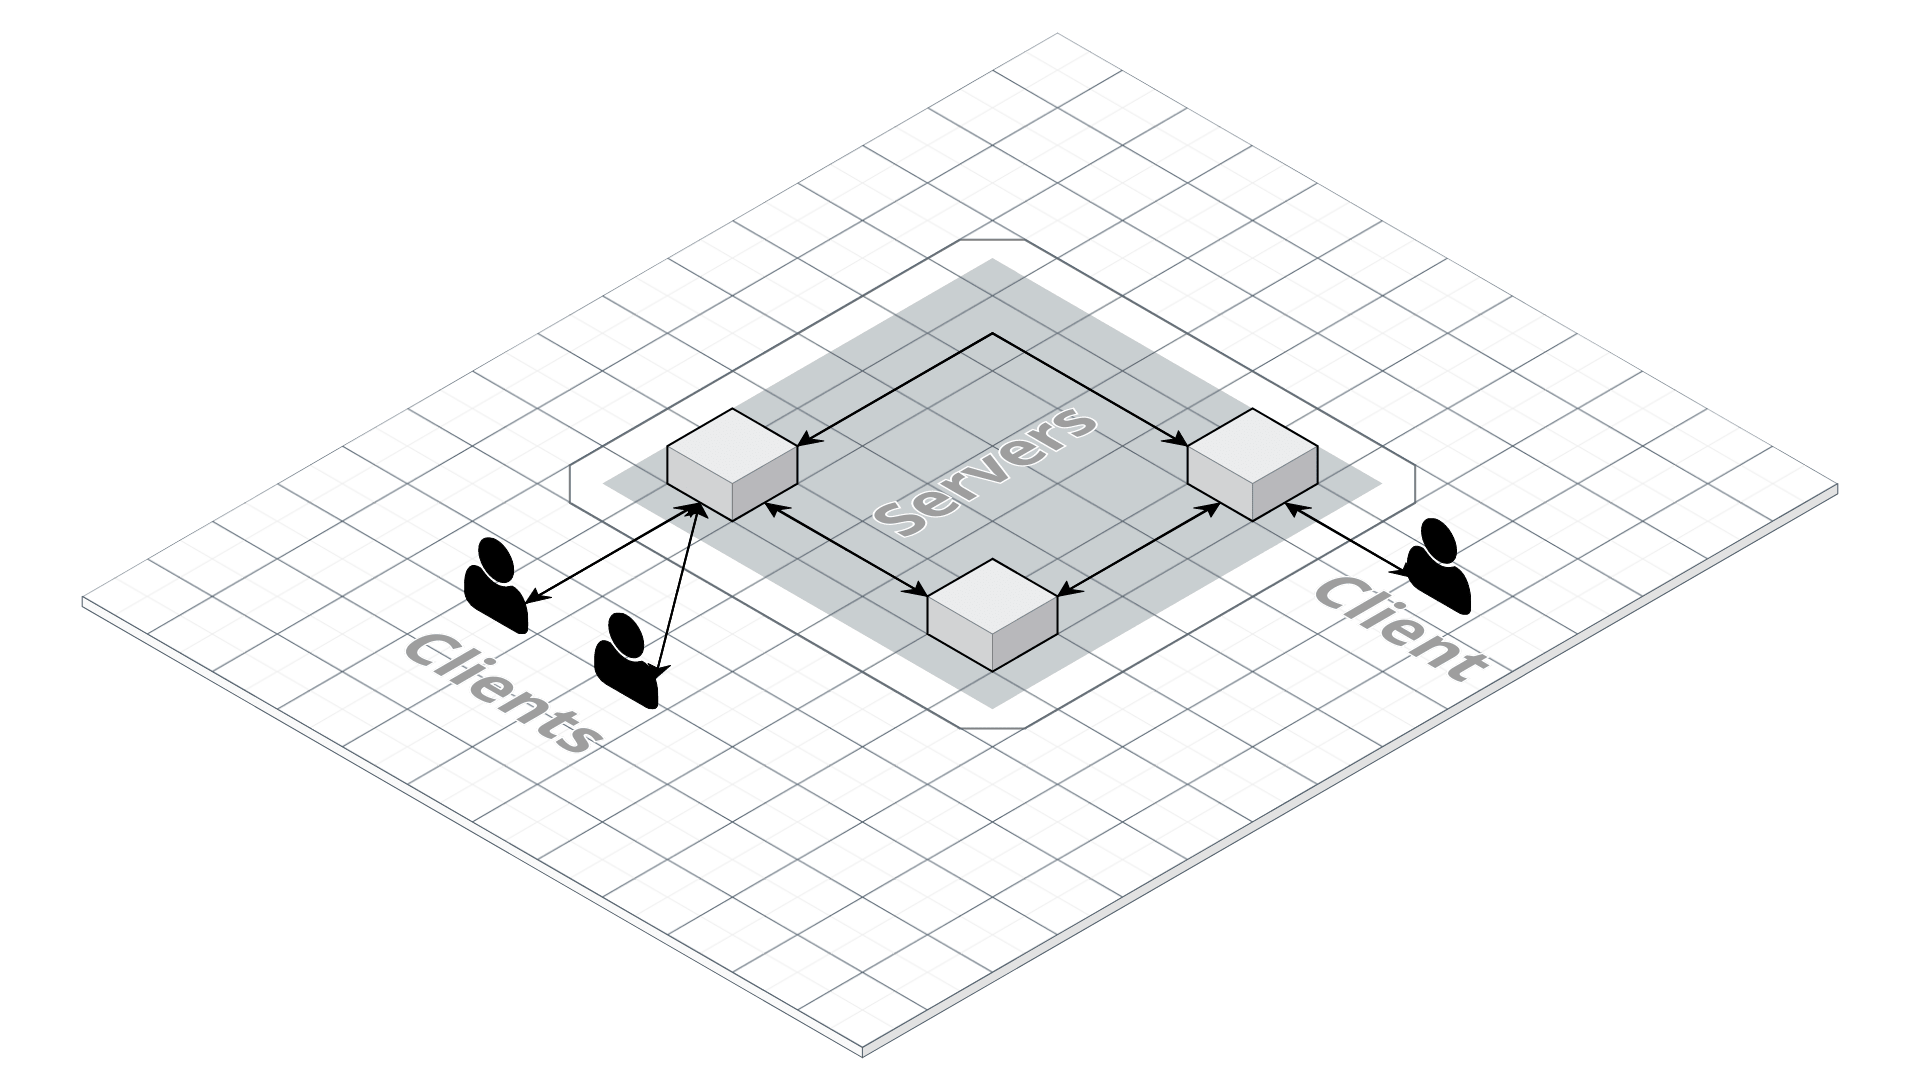
\includegraphics[width=\textwidth]{architecture.png}
    
    \caption{Architektur}
\end{figure}

\author{Matthias Vonend}
\subsection{Chatfunktionalität}
Damit ein Chat ablaufen kann, muss zunächst eine Verbindung zu einem Server aufgebaut werden.
Dazu wählt der Client zunächst einen zufälligen Server aus und versucht sich zu verbinden.
Wurde eine Verbindung erfolgreich aufgebaut, kann sich der Nutzer mit seinem Nutzername und seinem Password anmelden.
Sobald der Nutzer angemeldet ist, sendet der Server ihm alle benötigten Informationen inklusiver der verpassten
Nachrichten. Jede Nachricht hat ein Datum, wann es erstmalig an einem Server eingetroffen ist.
Anhand von diesem werden die Nachrichten sortiert, damit der Client die korrekte Reihenfolge darstellen kann.

Möchte dieser eine Nachricht an einen weiteren Client senden, schickt er diese an seine verbundene Node und
überlässt die Zustellung dieser. Da alle Nachrichten aus Persistenzgründen an alle Nodes verteilt werden müssen,
brauchen die Nodes keine Information über die Clients anderer Nodes. Im Falle einer solchen Anforderung
(z.\,B. Abfrage, ob ein anderer Nutzer aktiv ist) könnte ein Protokoll ähnlich zu Routing-Tabellen implementiert werden.
Empfängt eine Node eine Nachricht, egal ob von einem Client oder von einer anderen Node,
überprüft diese, ob die Nachricht für einen ihr bekannten Client bestimmt war und sendet diese gegebenenfalls an diesen.

//TODO Nach einer erfolgreichen Anmeldung kann der Nutzer
\author{Jan Grübener, Troy Keßler, Patrick Mischka, Michael Angermeier}
\subsection{Clientfunktionalitäten}
Nach einer erfolgreichen Anmeldung kann der Nutzer zwischen verschiedenen Funktionen auswählen.
\begin{enumerate}
    \item help
    \item chats
    \item contacts
    \item createchat
    \item openchat
    \item exit
\end{enumerate}
\paragraph{Funktion: help}
Diese Funktion ist nur im Command-Line-Client implementiert und gibt dem Nutzer einen Überblick
über alle möglichen Funktionen, die er aufrufen kann. Alle Funktionen sind in ein paar Worten beschrieben,
sodass der Benutzer gleich weiß, was diese Funktion genau macht.
\paragraph{Funktion: chats}
Bei einem Aufruf dieser Funktion werden alle Chats, die für den Nutzer zugänglich sind, angezeigt.
Dafür werden zunächst alle Chats durch die Methode getChats aus der API in einem Set aus Chats gespeichert.
Je nachdem, ob Chats verfügbar sind, bekommt der Benutzer unterschiedliche Antworten.
Sind keine Chats vorhanden, wird dies in einer Meldung angezeigt.
Sind Chats vorhanden, werden sowohl die Chatnamen als auch der/die User/s in diesem Chats angezeigt.
\paragraph{Funktion: contacts}
//TODO
\paragraph{Funktion: createchat}
Diese Funktion beginnt mit einer Aufforderung an den Benutzer, einen Chatnamen einzugeben.
Danach wird die Anzahl der Teilnehmer in dem Chat abgefragt. Diese muss mindestens 1 betragen.
Ist die Anzahl an Teilnehmern einmal gesetzt, müssen im nächsten Schritt alle Benutzernamen
der Teilnehmer eingetraggen werden. Hierfür wird jeder einzelener Benutzername abgefragt und
im Falle eines invaliden Benutzernamens, wird der Benutzer durch eine Meldung darauf aufmerksam gemacht.
Wurden alle 3 Attribute (Chatname, Teilnehmeranzahl, Username der Teilnehmer) erfolgreich eingegeben,
wird ein neuer Chat erstellt.
\paragraph{Funktion: openchat}
Auch hier muss der Benutzer zuerst den Chatnamen eingeben. Ist dieser vorhanden, wird der Chat geöffnet, ansonsten
bekommt der Benutzer wieder eine Meldung. Am Anfang eines Chats wird immer darauf hingewiesen, wie der Chat
verlassen werden kann. Danach werden alle Nachrichten, die in diesem Chat bereits geschrieben wurden, geladen.
Anschließend kann der Benutzer Nachrichten verschicken und empfangen.

\author{Matthias Vonend, Aaron Schweig, Troy Keßler}
\subsection{Fehlerbehandlung}
Aus den Anforderungen geht hervor, dass es mindestens zwei Server geben muss, die sämtliche Informationen des
Chatsystems besitzen müssen. Bricht eine Node zusammen muss dementsprechend eine andere Node dessen Aufgabe übernehmen.

\subsubsection{Client}
//TODO Troy

Im Fehlerfall scheitert das Senden einer Nachricht an den Server. In diesem Fall versucht sich der Client mit
einer anderen Node zu verbinden und sendet die Nachricht erneut.

\subsubsection{Server}
Serverseitig können verschiedene Fehler auftretten. VIele Fehler werden bereits durch das TCP-Protokoll verhindert.
Dennoch können grundsätzlich die folgende Fehlerfälle eintretten:
\begin{enumerate}
    \item Nachricht des Clients kann nicht korrekt empfangen/gesendet werden\\
        In diesem Fall muss der Server davon ausgehen, dass die Verbindung zusammengebrochen ist und er beendet
        seine Verbindung. Der Server verlässt sich darauf, dass der Client erneut eine Verbindung aufbaut.
        Alle für den Client relevanten Nachrichten werden dann zu diesem übertragen und der Client muss
        neue Informationen zurück übertragen
    \item Nachrichten einer Nachbarnode können nicht korrekt empfangen/gesendet werden\\
        Ähnlich zur Clientverbindung muss der Server davon ausgehen dass die Verbindung zusammengebrochen ist.
        Allerdings ist der Server hier selbst dafür zuständig sich erneut zu verbinden. Sämtliche Nachrichten,
        die an eine Node gesendet werden müssen werden in einer Queue aufbewahrt und nacheinander gesendet.
        Scheitert die Verbindung, so bleibt die Queue unverändert und wird nach einem erneuten Verbinden
        weiter abgearbeitet. Es wird solange versucht zu verbinden, bis eine Verbindung zustande gekommen ist.
        Sobald eine Verbindung wieder aufgebaut wurde synchronisieren sich die Nodes um wieder einen vollständigen
        Informationsstand zu besitzen.
        Sind keine Nachrichten zu senden, hat die Node keine Möglichkeit festzustellen,
        ob eine Verbindung noch existiert. Zu diesem Zweck existiert ein Heartbeat, der periodisch
        die Nachbarnodes anpingt und so prüft, ob die Verbindung noch existiert.
\end{enumerate}
Wie gerade beschrieben führen alle beteiligten stets eine synchronisation durch wodurch diese immer den kompletten Informationsbestand besitzen. Die Replikationskontrolle wird nach der Write-All-Available Strategie umgesetzt. Ein Client schickt eine Nachricht an einen Server, der versucht alle zu ihm verbundenen Nodes aktuell zu halten indem er die Nachricht oder die Änderung an alle verfügbaren Nodes weiterleitet.

Eine Veränderung des Datenbestandes muss dem entsprechend an alle anderen Nodes weiter gegeben werden.
Dadurch sind alle Server gleichwertige Servern.




